

	\begin{minipage}{0.5\linewidth}
		\section{Decken auf Wänden}
		
		\textbf{Flächentragwerke:}
			
			\begin{itemize}
				
				\item Scheibe
				
				\item Platte:
					
					\begin{itemize}
						
						\item Ebene, Tragwerk, Biegesteifigkeit EI > 0
						
						\item keine Belastung in Plattenebene
						
						\item Lagerung: Linienlagerung, Punktlagerung
						
						\item Lastabtrag in 2 Richtungen
						
					\end{itemize}
										
				
			\end{itemize}
		
		
	\end{minipage}
	\begin{minipage}{0.5\linewidth}
		
		\begin{itemize}
			
			\item Schale
			
			\item Faltwerk
			
			\item Fundamente
			
			\begin{itemize}
				
				\item Einzelfundamente
				
				\item Streifenfundamente
				
				\item Flachfundamente
				
			\end{itemize}
			$ \rightarrow $ elastisch gebettet auf dem Untergrund
			
			
		\end{itemize}
		
	\end{minipage}
	\begin{minipage}{0.5\linewidth}
		
		\subsection{Platten}
			
			\textbf{einachsig gespannte Platten:} \\
				freie Ränder oder Seitenverhältnis > $ \frac{1}{2} $ \\
				Bemessung wie Balken, meist Plattenstreifen 1m \\
				
			\textbf{zweiachsig gepsannte Platten:}	\\
				3-4 seitig gelagert, Seitenverhältnis < $ \frac{1}{2} $ \\
				bemessung als platte erforderlich \\
			
			
	\end{minipage}
\begin{minipage}{0.5\linewidth}
	
	 $ \frac{kN}{mm^2} \cdot 10^6 = \frac{kN}{m^2} $ 
	
	\begin{wrapfigure}{L}{0.3\linewidth}
		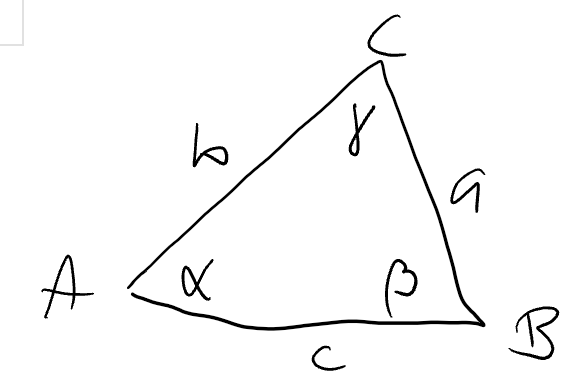
\includegraphics[width=\linewidth]{images/Dreieck.PNG}
	\end{wrapfigure}
	
	$ \frac{sin \gamma}{c} = \frac{sin \beta}{b} $ \\
	$ a^2 = b^2 + c^2 - 2bc \cdot cos \alpha $ \\
	$ b^2 = a^2 + c^2 - 2ac \cdot cos \beta $
	
\end{minipage}
	\begin{minipage}{0.65\linewidth}
		
		\subsubsection{\textcolor{red}{Elastische Plattentheorie} Schnittkräfte und Spannungen}
		
			\begin{tabular}{|lp{0.4\linewidth}|}
					
					\multicolumn{2}{c}{\textbf{Biegemomente und Normalkräft}} \\
					
					$ m_{x/y} = \int_{-h/2}^{+h/2} \sigma_{x/y} z \cdot dz \rightarrow \sigma_{x/y} = \frac{m_{x/y}}{I}z $	& \multirow{2}{*}{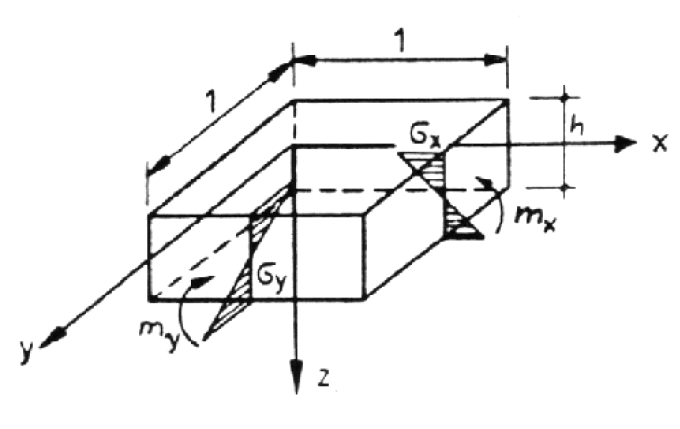
\includegraphics[width=\linewidth]{images/DW1Momente.PNG}}	\\
											 m$_x$ wirkt in x-Richtung, dreht um y-Achse  & \\
											 $ I = \frac{h^3}{12} $	 &  \\ \hline
					
					\multicolumn{2}{c}{\textbf{Drillmomente und Drillschubspannungen}} \\
					
					$ m_{xy} = \int_{-h/2}^{+h/2} \tau_{xy} z \cdot ds \rightarrow \tau_{xy} = \frac{m_{xy}}{I} z $		&	\multirow{2}{*}{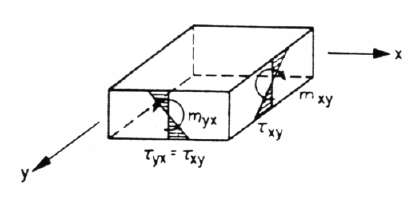
\includegraphics[width=\linewidth]{images/DW2Drillmomente.PNG}} \\
					
					$ \tau_{xy} = \tau_{yx} \rightarrow m_{xy} = m_{yx} $		& \\ \hline
					
					
					\multicolumn{2}{c}{\textbf{Querkräfte und Querschubspannungen}} \\
					
					$ \tau_{xz} = 1.5 \frac{\nu_x}{h} $		& \multirow{2}{*}{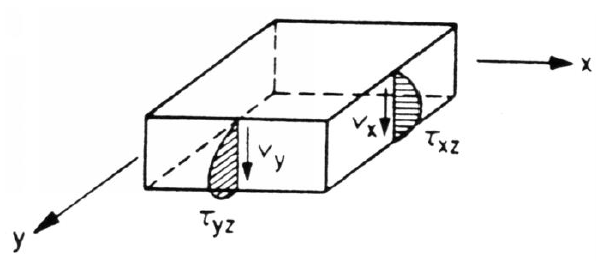
\includegraphics[width=\linewidth]{images/DW3Quer.PNG}} \\
					
					$ \tau_{yz} = 1.5 \frac{\nu_y}{h} $		& \\ \hline
					
			\end{tabular}
		
		
	\end{minipage}

	\begin{minipage}{0.55\linewidth}
		
		\subsubsection{Streifenmethode}
		
%		\begin{wrapfigure}{L}{0.4\linewidth}
			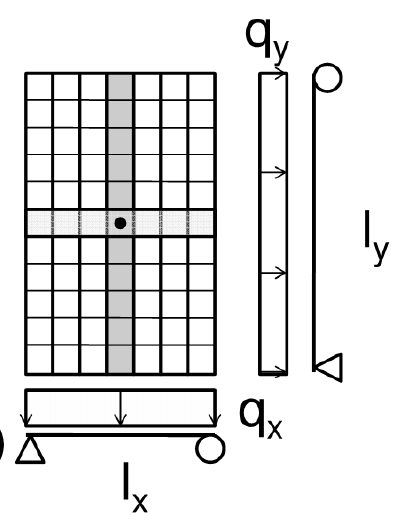
\includegraphics[width=0.4\linewidth]{images/DW4Achse.PNG}
%		\end{wrapfigure}
	
		Gleichgewicht: q = q$_x$ + q$_y$ \\
		Verträglichkeit: grösste Plattendruchbiegung: w$_x$ = w$_y$ \\
		$ \rightarrow w = \frac{M}{EI}; w_x = \frac{5 \cdot q_x \cdot l_x^4}{384 \cdot E \cdot I}  \rightarrow $ Verträglichkeit: $ q_x \cdot l_x^4 = q_y \cdot l_y^4 $ \\
		
	\end{minipage}
	\begin{minipage}{0.4\linewidth}
		
		
		
		\subsubsection{Plattentafeln}
		
		\begin{itemize}
			
			\item Czerny: 3-/4-seitig gelagert, Gleichlasten, Querdehnung = 0
			
			\item Stiglat/Wippel: versch. Lasten und Lagerungen, drillsteif
			
			\item Pieper/Martens: Drillsteif und drillweich, Angaben für Z'swirken angrenzender Platten
			
		\end{itemize}
		
	\end{minipage}

	\begin{minipage}{0.5\linewidth}
		
		\subsubsection{Querdehnung}
			\textbf{Drillsteife Quadratplatte nach elastischer Plattentheorie, Eckkräfte} 
			
			$ \rightarrow $ Drillmomente haben grosse Momente und konzentrierte Reaktionen im Eckbereich zur Folge \\
			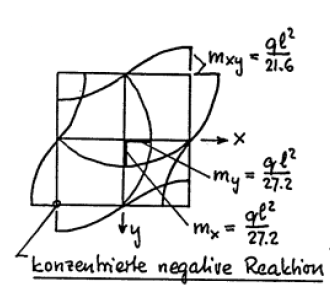
\includegraphics[width=0.5\linewidth]{images/DW5Querdehnung.PNG} 
			
			$ \rightarrow $ Falls keine Eckkräft aufgenommen werden können, entstehen kleinere Drillmomente und grössere Feldmoment \\
			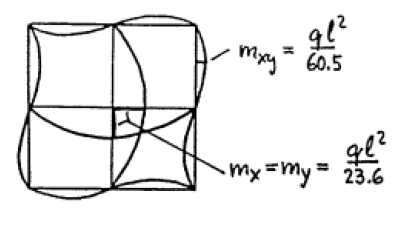
\includegraphics[width=0.5\linewidth]{images/DW6Querdehnung.PNG}
			
			$ \rightarrow $ Insbesondere Decken über dem obersten Geschoss können öft nicht in der Ecke verankert werden \\
			
			\textbf{Annahme: Platte mit elastischer Biegesteifigkeit, ohne Drillsteifigkeitm Durchbiegungsverträglichkeit an jedem Punkt erfüllt}
			
			$ \rightarrow $ Momente in Feldmitte $ m_x = m_y = \frac{q \cdot l^2}{12} \Rightarrow $ viel grössere Momente und Durchbiegung \\
		
	\end{minipage}
	\begin{minipage}{0.5\linewidth}
		

		
		\textbf{Durchlaufende Platten:}
			\begin{itemize}
						
				\item Rechteckplatten mit beliebigen Stützweitenverhältnisse $ \rightarrow $ Berechnung nach Pieper/Martens
				
				\item Rechteckplatten mit geringen Stützweitenunterscheiden (l$_{min}$/l$_{max}$ > 0.75) $ \rightarrow $ Belastungsumordnungsverfahren
				
			\end{itemize}
%\textcolor{red}{Vorlesung 04, Folie 8}
		
		\subsubsection{Auflagerreaktionen}
		
		Entlang Bruchlinie Einzugsgebiete bestimmen $ \rightarrow $ Einzugsgebietsflächen wirken je auf ein Auflager
		
		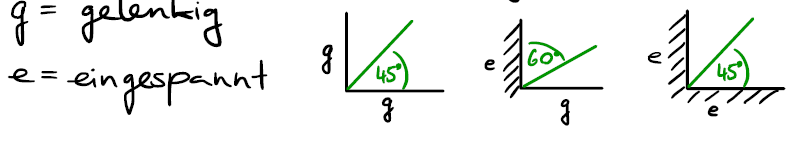
\includegraphics[width=\linewidth]{images/DW7Auflagerreaktion.PNG}
		
		
		durchgehende Wände: $ q_i = A_i \frac{1}{l} q_d \frac{1}{1m} [\frac{kN}{m^l} ] \rightarrow \cdot l [kN] $ \\
		
		mit z.B. Fenster: $ q_i = A_i \frac{l_i}{l} q_d \frac{1}{1m} [\frac{kN}{m^l} ]  \rightarrow \cdot l_x [kN] $
		
		
		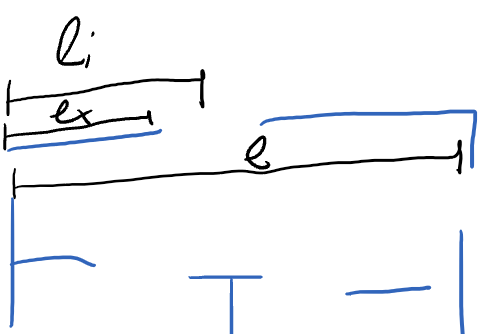
\includegraphics[width=0.7\linewidth]{images/DW8Auflagerlange.PNG}
		
	\end{minipage}

%	\begin{minipage}{0.5\linewidth}
%		
%		\subsubsection{Auflagerreaktionen}
%		
%		Entlang Bruchlinie Einzugsgebiete bestimmen $ \rightarrow $ Einzugsgebietsflächen wirken je auf ein Auflager
%		
%		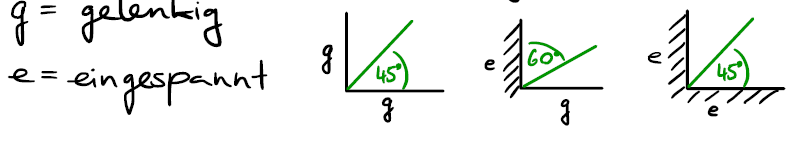
\includegraphics[width=\linewidth]{images/DW7Auflagerreaktion.PNG}
%		
%		
%	\end{minipage}
	\begin{minipage}{\linewidth}
		\begin{multicols}{2}
			
			

		\subsubsection{Bewehrung}
		
		Querkraftbemessung: SIA 262 4.3.3.1.3 $ \rightarrow $ Gl. 35 erfüllt, Mindestbewehrung bei dünnen Platten nicht nötig \\
		
		Biegebewehrung: SIA 262 5.5.3 \\
		
		Drillbewehrung: bei drillsteif berechneten Platte (z.b. Czerny) $ \rightarrow $ Drillweich: mehr Biegemomente \& Verformung \\
		
		Bewehrung bei Aussparung: 
			\begin{itemize}
				
				\item kleine Öffnung (bis zu doppelter Plattendicke): kein wesentlicher Einfluss auf Tragverhalten
				
				\item mehrere kleine Öffnungen ungünstige Anordnung oder schmale Schlitze: Wirkung wie grosse Öffnung
				
				\item mehrere kleine Öffnungen in Plattenecken: Verlust Drillsteifigkeit (mehr Feldmomente)
				
				\item  mittlere Öffnungen: geringer Einfluss auf Tragverhalten (konstruktive Massnahmen mit erhöhtem Aufwand)
				
				\item mittlere Öffnungen z.b. Kamine: Ober- und Unterseite der Platte separat betrachten
				
				\item grosse Öffnungen (z.b. Treppen): konstruktivee Massnahmen basierend auf rechnerischem Nachweis
				
			\end{itemize}
		
		\end{multicols}
	\end{minipage}
